\chapter{Introduction}

%Workflow is becoming popular

Over the years, with the emerging of the fourth paradigm of science discovery \cite{Hey2009}, scientific workflows continue to gain their popularity among many science disciplines, including physics \cite{Deelman2002}, astronomy \cite{Sakellariou2010}, biology \cite{Lathers2006, Oinn2004}, chemistry \cite{Wieczorek2005}, earthquake science \cite{Maechling2007} and many more. Scientific workflows increasingly require tremendous amounts of data processing and workflows with up to a few million tasks are not uncommon \cite{Callaghan2011}. Among these large-scale, loosely-coupled applications, the majority of the tasks within these applications are often relatively small (from a few seconds to a few minutes in runtime). However, in aggregate they represent a significant amount of computation and data \cite{Deelman2002}. For example, the CyberShake workflow \cite{Rynge2012} is used by the Southern California Earthquake Center (SCEC) \cite{SCEC} to characterize earthquake hazards using the Probabilistic Seismic Hazard Analysis (PSHA) technique. CyberShake workflows composed of more than 800,000 jobs have been executed on the TeraGrid \cite{TeraGrid}. When executing these applications on a multi-machine parallel environment, such as the Grid or the Cloud, significant system overheads may exist. An overhead is defined as the time of performing miscellaneous work other than executing the user's computational activities.  Overheads may adversely influence runtime performance \cite{Overhead2011}. In order to minimize the impact of such overheads, task clustering \cite{Singh2008,Hussin2010,Zhao2009} has been developed to merge small tasks into larger jobs so that the number of computational activities is reduced and their computational granularity is increased thereby reducing the (mostly scheduling related) system overheads. %Task clustering has been widely used in executing such large-scale scientific workflows and has demonstrated its great effort \cite{Rynge2012}. 

\begin{figure}[h!]
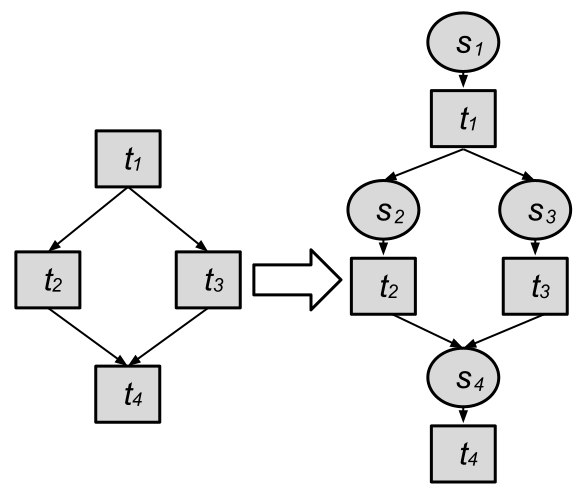
\includegraphics[width=0.5\linewidth]{figures/introduction/odag.png}
\centering
  \captionof{figure}{Extending DAG to o-DAG}
  \label{fig:intro_odag}
\end{figure}

Traditionally a workflow is modeled as a Directed Acyclic Graph (DAG). Each node in the DAG represents a workflow task, and the edges represent dependencies between the tasks ($t$) that constrain the order in which the tasks are executed. Each task is a program and a set of parameters that need to be executed. A job ($j$) is a single execution unit and it contains one or multiple task(s). The dependencies typically represent data flow dependencies in the application, where the output files produced by one task are needed as inputs of another task. In this work, we extend the DAG model to be overhead aware (o-DAG). The reason is that system overheads play an important role in workflow execution and they constitute a major part of the overall runtime when tasks are poorly clustered. Fig~\ref{fig:intro_odag} shows how we augment a DAG to be an o-DAG with the capability to represent scheduling overheads ($s$) such as workflow engine delay, queue delay, and postscript delay. The classification of overheads is based on the model of a typical workflow management system shown in Fig~\ref{fig:intro_system}. The components in this WMS are listed below: 

\begin{figure}[h!]
\centering
  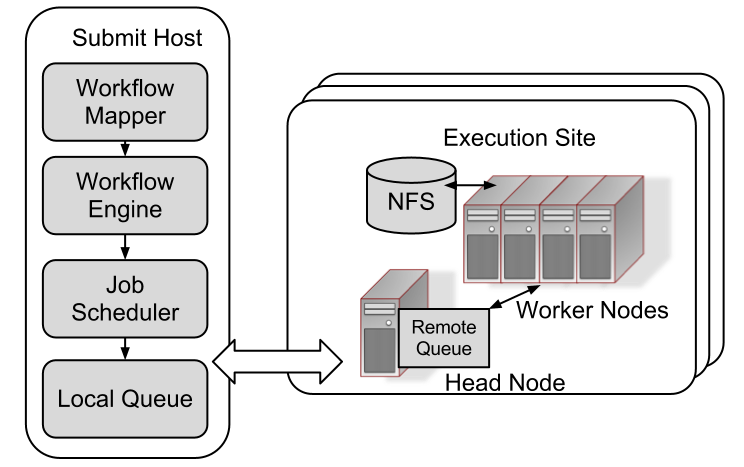
\includegraphics[width=0.6\linewidth]{figures/introduction/system.png}

  \caption{System Model}
  \label{fig:intro_system}
\end{figure}


\textbf{Workflow Mapper} generates an executable workflow based on an abstract workflow provided by the user or workflow composition system. 

\textbf{Workflow Engine} executes the jobs defined by the workflow in order of their dependencies. Only free jobs that have all their parent jobs completed are submitted to  Job Scheduler. 

\textbf{Job Scheduler} and \textbf{Local Queue} manage individual workflow jobs and supervise their execution on local and remote resources.

\textbf{Job Wrapper} extracts tasks from clustered jobs and executes them at the worker nodes. 


\begin{figure}[h!]
\centering
 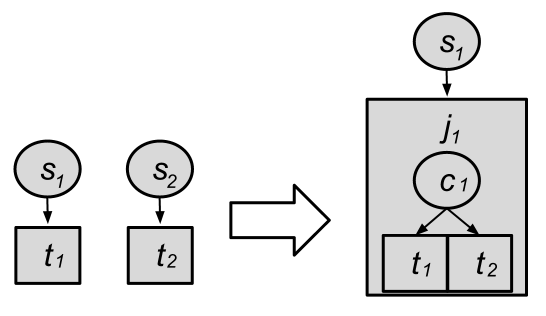
\includegraphics[width=0.6\linewidth]{figures/introduction/hc.png}
  \captionof{figure}{Task Clustering}
  \label{fig:intro_hc}
\end{figure}

%This classification of scheduling overheads is based on our prior studies on workflow analysis \cite{Overhead2011}. 

%Clustering delay ($c$) measures the difference between the sum of the actual task runtime and the job runtime seen by the job scheduler. The cause of clustering delay is usually the use of a job wrapper to execute a clustered job. 
%The job wrapper takes some time to extract the list of tasks and to launch them.

With o-DAG model, we can explicitly express the process of task clustering. For example, in Fig~\ref{fig:intro_hc}, two tasks $t_1$ and $t_2$ without data dependency between them are merged into a clustered job $j_1$. Scheduling overheads ($s_2$) are reduced but clustering delay ($c_1$) is added. 

%After horizontal clustering, $t_1$ and $t_2$ in $j_1$ can be executed in sequence or in parallel if supported. In this paper, they are executed in sequence. Given one available resource, the overall runtime for the workflow (left) is $runtime_1=s_1+t_1+s_2+t_2$ , and the overall runtime for the workflow (right) is $runtime_2=s_1+c_1+t_1+t_2$.  $runtime_1>runtime_2$ as long as  $c_1<s_2$ which is true in many distributed systems since the clustering delay within a worker node is usually smaller than the scheduling overhead across different worker nodes.  


%In a DAG model, nodes represent computational activities that users want to perform. Directed edges represent control or data dependencies that must be followed between the nodes. The simplicity and  expressivity of DAG wins wide support in many workflow management systems. In this work, we focus on the extension of DAG model to be overhead aware (o-DAG). An overhead is defined as the time of performing miscellaneous work other than executing the user's computational activities. 
%In general, the execution environment of high-performance computing systems is modeled as a resource pool of multiple computational units (nodes or cpu slots namely). This is usually true when it is limited to campus-wide clusters in universities or government labs, which are typically owned, maintained, and used by a single organization. However, in recent years, two new distributed computing paradigms require a more hierarchical model of execution environments with distributed computing resources. The development of grid computing \cite{Foster2004} has enabled virtual organizations (VO) to securely share the computational infrastructure of their member institutions. More recently, the emergence of cloud computing \cite{Armbrust2009} has made it possible to easily lease large-scale computing infrastructure from commercial resource providers. However, with the increase of cloud computing. Scheduling problem is simplified as a clustering problem. 


%These developments have introduced many challenges for the management of large-scale scientific workflows. In this work, we generalize these requirements to the following research challenges:

In this work, we identify the new challenges when executing complex scientific applications:

The first challenge users face when merging workflow tasks is the \textbf{imbalance of computation}. Tasks may have diverse runtimes and such diversity may cause significant load imbalance. To address this challenge, researchers have proposed several approaches. Bag-of-Tasks \cite{Hussin2010, Celaya2010, Oprescu2010} dynamically groups tasks together based on the task characteristics but it assumes tasks are independent, which limits its usage in scientific workflows. Singh \cite{Singh2008} and Rynge \cite{Rynge2012} examine the workflow structure and groups tasks together into jobs in a static way for best effort systems. However, this work ignores the computational requirement of tasks and may end up with an imbalanced load on the resources. A popular technique in workload studies to address the load balancing challenge is over-decomposition \cite{Lifflander2012}. This method decomposes computational work into medium-grained tasks. Each task is coarse-grained enough to enable efficient execution and reduce scheduling overheads, while being fine-grained enough to expose significantly higher application-level parallelism than that is offered by the hardware. 

The second challenge has to do with the \textbf{data management within a workflow}. Scientific applications are often data intensive and usually need collaborations of scientists from different institutions, hence application data in scientific workflows are usually distributed. Particularly with the emergence of grids and clouds, scientists can upload their data and launch their applications on scientific cloud workflow systems from anywhere in the world via the Internet. However, merging tasks that have input data from or have output data to different data centers is time-consuming and inefficient. Merging tasks that have no intermediate data between them seems safe at the first sight. However, the subsequent tasks that rely on the output data that their parent tasks produce may suffer a data locality problem since data may be distributed poorly and the data transfer time is increased. Communication-aware scheduling \cite{Sonmez2006, Jones2004} has taken the communication cost into the scheduling/clustering model and have achieved some significant improvement. The workflow partitioning approach \cite{Hedayat2009, Yuan2010, Wieczorek2005,Rubing2005} represents the clustering problem as a global optimization problem and aims to minimize the overall runtime of a graph. However, the complexity of solving such an optimization problem does not scale well. Heuristics \cite{Maheshwari2012, Callaghan2010} are used to select the right parameters and achieve better runtime performance but the approach is not automatic and requires much experience in distributed systems. 
%However, what makes this problem even challenging is that solutions to address the data dependency challenge usually conflicts Therefore, we claim that it is necessary to consider the data dependencies with subsequent tasks (not only child tasks). However, they have forgotten balance and data structure problem. 


\textbf{Resource management} is the third challenge that is brought by the recent emergence of cloud computing and resource provisioning techniques. Along with the increase of the scale of workflows, the number and the variety of computational resources to use has been increasing consistently. Infrastructure-as-a-Service (IaaS) clouds offer the ability to provision resources on-demand according to a pay-per-use model and adjust resource capacity according to the changing demands of the application \cite{Abrishami2012}. Task clustering can still be applied to this cloud scenario \cite{Deelman2010, Vockler2011}. However, the decisions required in cloud scenarios not only have to take into account performance-related metrics such as workflow makespan, but must also consider the resource utilization, since the resources from commercial clouds usually have monetary costs associated with them. Therefore, the adoption of task clustering on cloud computing requires the development of new methods for the integration of task clustering and resource provisioning. 

%Fault Tolerance Challenge
The fourth challenge has to do with \textbf{fault tolerance}. Existing clustering strategies ignore or underestimate the impact of the occurrence of failures on system behavior, despite the increasing impact of failures in large-scale distributed systems. Many researchers \cite{Zhang2004, Tang1990, Schroeder2006, Sahoo2004} have emphasized the importance of fault tolerance design and indicated that the failure rates in modern distributed systems are significant. The major concern has to do with transient failures because they are expected to be more prevalent than permanent failures \cite{Zhang2004}. For example, denser integration of semiconductor circuits and lower operating voltage levels may increase the likelihood of bit-flips when circuits are bombarded by cosmic rays and other particles \cite{Zhang2004}. In a faulty environment, there are usually three approaches for managing workflow failures. First, one can simply retry the entire job when its computation is not successful as in the Pegasus Workflow Management System \cite{Deelman2004}. However, some of the tasks within the job may have completed successfully and it could be a waste of time and resources to retry all of the tasks. Second, the application process can be periodically check-pointed so that when a failure occurs, the amount of work to be retried is limited. However, the overheads of checkpointing can limit its benefits \cite{Zhang2004}. Third, tasks can be replicated to different nodes to avoid location-specific failures \cite{Zhang2009}. However, inappropriate clustering (and replication) parameters may cause severe performance degradation if they create long-running clustered jobs. 
%Intuitively, a long-running job that consists of many tasks has a higher job failure rate even when the overall task failure rate is low. 

% Many many citations

After examining the major challenges in executing large-scale scientific workflows, we contribute to the studies of workflow performance improvement through task clustering in the following aspects:

First of all, we \textbf{extend the existing DAG model to be overhead aware} and quantitatively analyze the relationship between the workflow performance and overheads. Previous research has established models to describe system overheads in distributed systems and has classified them into several categories \cite{Prodan2007, Prodan2008}. In contrast, we investigate the distributions and patterns of different overheads and discuss how the system environment (system configuration, etc.) influences the distribution of overheads. Furthermore, we present quantitative metrics to measure and evaluate the characters (robustness, sensitivity, balance, etc.) of workflows. Finally, we analyze the relationship between these metrics and the workflow performance with different optimization methods. 

Second, to \textbf{solve the computation imbalance problem}, we introduce a series of balanced clustering methods. The computation imbalance problem means that the execution of workflows suffers from significant overheads (unavailable data, overloaded resources, or system constraints) due to inefficient task clustering and job execution. We identify the two challenges: runtime imbalance due to the inefficient clustering of independent tasks and dependency imbalance that is related to dependent tasks. What makes this problem even more challenging is that solutions to address these two problems are usually conflicting. For example, balancing runtime may aggravate the dependency imbalance problem, and vice versa. A quantitative measurement of workflow characteristics is required to serve as a criterion to select and balance these solutions. To achieve this goal, we propose four metrics to reflect the internal structure (in terms of runtime and dependency) of the workflow. 

Third, we introduce \textbf{data aware workflow partitioning} to reduce the data transfer between clustered jobs. Data-intensive workflows require significant amount of storage and computation. For these workflows, we need to use multiple execution sites and consider their available storage. Data aware partitioning aims to reduce the intermediate data transfer in a workflow while satisfying the storage constraints. Heuristics and algorithms are proposed to improve the efficiency of partitioning and experiment-based evaluation is performed to validate its effectiveness.  


Fourth, we propose \textbf{fault tolerant clustering} that dynamically adjusts the clustering strategy based on the current trend of failures. We classify transient failures into two categories, task failure and job failure and furthermore indicate their distinct influence on the overall performance. During the runtime, this approach estimates the failure distribution among all the resources and dynamically merges tasks into jobs of moderate size and recluster failed jobs to avoid failures.

Finally, to achieve a resource aware clustering in scientific workflows, we propose to \textbf{integrate resource provisioning with task clustering}. We first analyze the relationship between the overall runtime of a clustered job and the allocated resources (CPU, memory, and storage). Then we develop resource aware clustering algorithms to partition a workflow and predict the number of cores and wall time required for each partition. Furthermore,  we integrate the clustering algorithms with resource provisioning and develop an estimation method to be used to provision VMs on a cloud and predict the cost of running the workflow. We also investigate the scenario when resources are constrained (such as storage) and propose algorithms and heuristics to improve the workflow performance. 

%The less the better


Overall, this thesis aims to \textbf{improve the overall performance of task clustering in large-scale scientific workflows}. We present both experiment-based and simulation-based evaluation of a wide range of scientific workflows. 
 
%In particular, we provide a novel approach to capture these metrics. Our work considers the neighboring tasks including siblings, parents, children and so on because such a family of tasks has strong connections between them. The performance evaluation shows that they can significantly reduce the imbalance problem and we analyze and connect the performance of these metrics and balancing methods. These quantitative metrics indicate which type of imbalance problem a workflow is more likely to suffer from. Comparing the relative values of these metrics informs the selection of a balancing method or a combination of these methods. 

%The Pegasus Workflow Management System (Pegasus WMS) is a framework for mapping complex workflows onto distributed resources such as grids and clouds. Pegasus has been used to optimize runtime performance of various scientific applications in astronomy, biology, physics, and earthquake science on dedicated clusters, and national cyberinfrastructure such as the TeraGrid and the Open Science Grid. To prepare and execute a large-scale workflows on these distributed environments has features such as the distributed nature of these resources, the large number of tasks in a workflow, and the complex dependencies among the tasks. Due to these features, significant overheads can occur during workflow execution. Failures occurring to different layers of the workflow management systems may exist. These challenges are hard to solved with conventional scheduling algorithm based approach. Instead, we aim to use a workflow restructuring approach that reorganizes workflow activities within it to improve the resource utilization, runtime performance and fault tolerance. For example, many of existing algorithms have ignored or underestimated the overheads and runtimes variabilities. 

